\documentclass{report}

%%METADATA
\title{Inventor Moves from the most Innovative Firms to the Laggard Firms  }
\author{
Raman Singh Chhina \\ {University of Chicago}
}
\date{}

%%PACKAGES
\usepackage{graphicx}
\usepackage{tabularx}
\usepackage{setspace}
\usepackage{amsmath,amsthm,amssymb}
\usepackage[hyphens]{url}
\usepackage{natbib}
\usepackage[font=normalsize,labelfont=bf]{caption}
\usepackage[margin=1in]{geometry}
\usepackage{hyperref}
\hypersetup{colorlinks=true,urlcolor=blue,citecolor=red}
\usepackage{enumerate}% http://ctan.org/pkg/enumerate %Supports lowercase Roman-letter enumeration
\usepackage{verbatim} %Package with \begin{comment} environment
\usepackage{physics}
\usepackage{tikz}
\usepackage{listings}
\usepackage{upquote}
\usepackage{booktabs} %Package with \toprule and \bottomrule
\usepackage{etoc}     %Package with \localtableofcontents
\usepackage{multicol}
\usepackage{bm}
\usepackage{float}
%\usepackage[framemethod=TikZ]{mdframed}

\definecolor{dkgreen}{rgb}{0,0.6,0}
\definecolor{gray}{rgb}{0.5,0.5,0.5}
\definecolor{mauve}{rgb}{0.58,0,0.82}

\lstset{language=bash,
  frame=tb,
  aboveskip=3mm,
  belowskip=3mm,
  showstringspaces=false,
  columns=flexible,
  basicstyle={\small\ttfamily},
  numbers=none,
  numberstyle=\tiny\color{gray},
  keywordstyle=\color{blue},
  commentstyle=\color{dkgreen},
  stringstyle=\color{mauve},
  breaklines=true,
  breakatwhitespace=false,
  tabsize=3
}
\newtheorem{theorem}{Theorem}
\newtheorem{lemma}[theorem]{Lemma}
\newtheorem{proposition}[theorem]{Proposition}

%%FORMATTING
\onehalfspacing
\numberwithin{equation}{section}
\numberwithin{figure}{section}
\numberwithin{table}{section}
\bibliographystyle{bib/aeanobold-oxford.bst}

\usepackage{beramono}
\usepackage{listings}
\usepackage[usenames,dvipsnames]{xcolor}


%LOGBOOK
\begin{document}

%%LOGBOOK COVER
\maketitle

%TABLE OF CONTENTS
%\renewcommand{\thechapter}{\Alph{chapter}}
\setcounter{tocdepth}{1}
\tableofcontents
\etocsettocstyle{}{} % from now on only local tocs

\clearpage
\section{Overview}

This exercise looks at the trends in knowledge diffusion in US firms by focusing on the moves of inventors between firms. Specifically, I plot the fraction of the total moves that constitute an inventor moving from a highly innovative firm to a laggard firm for each year since 1980. The results are shown in Fig~\ref{fig:f1} and \ref{fig:f2}

\section{Data}

I use USPTO data from the PatentsView website. The data begins in the year 1980.

\section{Methodology}

\subsection{Definition of top one percent}
Right now I'm using an ex-post definition of most innovative firms i.e. the firms are ranked based on their total patents between \underline{1980 to 2018}. This ranking is kept constant for each year. Sina suggested to rank the firms for year $t$ based on their total patents between years $t$ and $t-10$. This limits the range to 1990-2018 using the PatentsView data. \textcolor{blue}{Could you suggest another source which can be linked to PatentView for historical patents?}

\subsection{What is a move?}
An inventor is deemed to have moved at date $t$ if the assignee firm on the patent granted at time $t$ is different from the assignee firm on the immediately preceding patent. Note that
\begin{enumerate}
    \item To register a move, the inventor must be observed at least twice
    \item A move is registered only when the inventor is granted a patent.
    \item This wouldn't capture the moves from top to laggard firms if the inventor doesn't registers a patent after moving to a laggard firm. 
\end{enumerate}

\section{Results}

The results are plotted in Fig~\ref{fig:f1} and \ref{fig:f2}. The fraction shows a sharp decline in the 1990 to 2010 period and is rising in the rest of the horizon. 
\begin{figure}
    \centering
    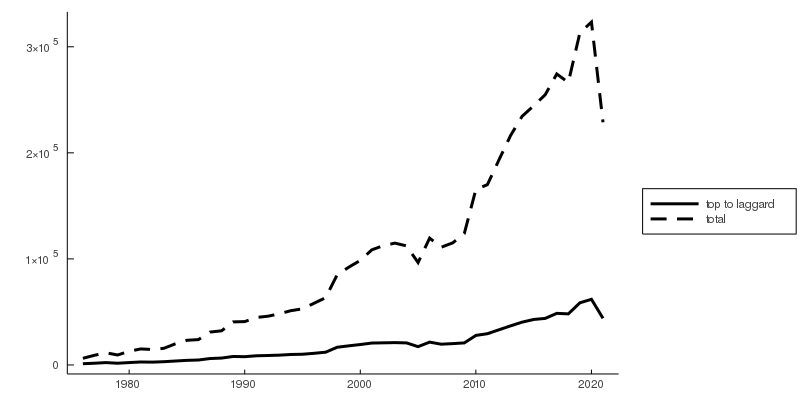
\includegraphics[width = 0.8\textwidth]{input/total_moves.png}
    \caption{Total moves of inventors between firms and number of moves from top one percent to the rest}
    \label{fig:f1}
\end{figure}

\begin{figure}
    \centering
    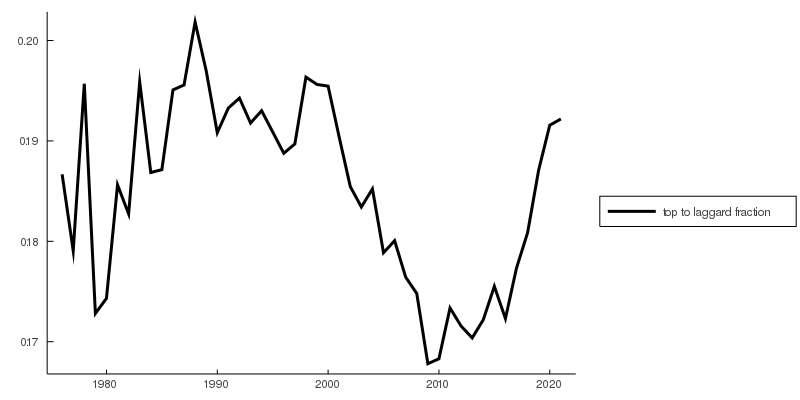
\includegraphics[width = 0.8\textwidth]{input/fraction.png}
    \caption{Fraction of the moves that are from top one percent to the rest of the firms}
    \label{fig:f2}
\end{figure}

\section{Code}

The LaTeX and Julia code can be accessed in the Github repo \href{https://github.com/econ-raman/code_share/tree/main/patent_exercise}{here}.
%%LOGBOOK BIBLIOGRAPHY
\bibliography{bib/reference.bib}

\end{document}
